%%%%%%%%%%%%%%%%%%%%%%%%%%%%%%%%%%%%%%%%%%%%%%%%%%%%%%%
% A template for Wiley article submissions.
% Developed by Overleaf. 
%
% Please note that whilst this template provides a 
% preview of the typeset manuscript for submission, it 
% will not necessarily be the final publication layout.
%
% Usage notes:
% The "blind" option will make anonymous all author, affiliation, correspondence and funding information.


\documentclass[num-refs]{wiley-article}


% Add additional packages here if required
\usepackage{siunitx}
\usepackage{float}
\usepackage{adjustbox}

\title{Complex data - final project: \\Analysis of kidney condition}



\author[1]{Anna Zaleska}
\author[1]{Stanisław Wilczyński}



% Include full affiliation details for all authors
\affil[1]{Univeristy of Wrocław}

\corraddress{Univeristy of Wrocław}
\corremail{sjwilczynski@gmail.com, aniazaleska1@gmail.com}


\begin{document}

\maketitle


\begin{abstract}
In this project we analyze the medical data on kidney condition after transplant measured repeatedly after surgery available in \cite{PBImisc}. We fit and compare mixed and fixed effects models, interpret them and examine their effectiveness in terms of prediction.  

\keywords{longitudinal data, medical data, mixed effects, fixed effects, neural network}
\end{abstract}

\tableofcontents

\section{Introduction}

\subsection{The data set}

\paragraph{Covariates}
The obtained data set consists of information about kidney condition in time after the transplant surgery. The data was gathered based on 334 patients' observations.  We can divide the covariates of the data set into two groups:
\begin{itemize}
\item Time measurements 

Statistics of MDRD in 8 different time points: 7, 30 days and 3, 6, 12, 24, 36 and 60 months after kidney transplant. MDRD (Modification of Diet in Renal Disease) is an estimator of glomerular filtration rate (GFR) from serum creatinine, which is used as a kidney condition indicator.  

\item Other characteristics
\begin{itemize}
\item recipient.age - age of the recipient at time of the surgery
\item donor.age - age of the donor at time of the surgery
\item CIT - Cold ischemia time - time that passed between taking the kidney from donor's body and introducing it to recipient's body
\item discrepancy.AB - number of discrepancies in AB antibodies
\item discrepancy.DR - number of discrepancies in DR antibodies
\item therapy - one of three different schemes of immunosuppression therapy
\item diabetes - the information if the recipient is diabetic
\item bpl.drugs -  number of drugs for blood pressure lowering
\end{itemize}
\end{itemize}

\paragraph{Time variable}

Although in the first approach (most general model) we use time as a factor, due to quite big number of time points $(8)$ we consider time as continuous variable also. However, the intervals between following time measurements are growing exponentially. Therefore, it may be better to build models based on the logarithm of time to make the gaps between measurements more balanced. Another premise for taking logarithm of time as explanatory variable are the means of the MDRD in time. They are $24.36, 47.27, 50.49$, $51.20, 52.22,$ $53.72, 53.74, 54.83$ for $7, 30$ days, $3,6,12$,$24,36,60$ months respectively. We can see that most variability (at least in the means) is in first half of the measurements, so for the models with not transformed time as explanatory continuous variable we could get corrupted models. We also compare these two options graphically. Below for chosen patients we plot their values of MDRD at all time points and fit a linear and quadratic regression with time as explanatory variable: not transformed on the upper plot, logarithm of time on the lower plot.
\begin{figure}[H] 
\centering
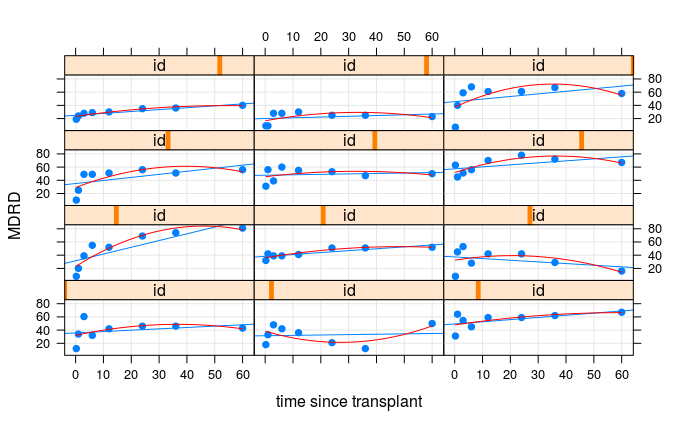
\includegraphics[height=0.4\textheight, width=\textwidth]{pictures/time.png}
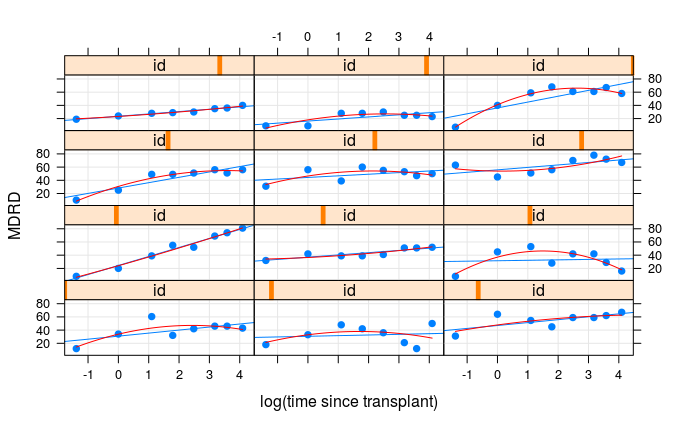
\includegraphics[height=0.4\textheight, width=\textwidth]{pictures/ltime.png}
\caption{Linear time vs. logarithm of time for patients $151-162$} \label{timePlot}
\end{figure}

As expected the curves on the upper plot do not fit the first three measurements very well, because their values differ significantly but they are very close on the X-axis. As a result of these arguments, we decide to include logarithm of time as explanatory variable in further analysis. From the plots above we can also conclude that the change of the kidney's efficiency is different for different patients - for example for some patients the dependency is linear and for other quadratic. Therefore fitting polynomial parametric curves can be plausible. 

\subsection{Aims of the analysis}
The exploration of obtained data set is focused on several main goals:
\begin{itemize}
\item Exploring how the condition of kidney after transplant depends on passing time

During our analysis we fit models with different time structures, considering time as factor, continuous variable and including random effects in order to find model(s) that best explain the dependence on time and interpret it.
\item Finding the key patients' characteristics that may influence the function of kidney

We want to know which of the examined characteristics have a significant impact on kidney condition and discover if the impact is positive or negative.
\item Studying group interactions between the factors presented in the data and time.
We would like to know how the additional characteristics interact with time and if there is a difference between changes in kidney condition in different groups of patients.


\end{itemize}
To achieve these goals we fit a wide range of models including both fixed and mixed effects. We test the models to find ones that best explain the influence of time and other characteristics on examined kidney condition. We compare proposed models using different criterion to make the analysis comprehensive.

\section{Fixed effects models}

In this section we fit a fixed effects model to our data as in the lecture and \cite[Chapters 5-7]{ALA}.

\subsection{Most general model}

First of all we have to choose the structure of our most general model. Firstly we incorporate the time as factor. Unfortunately because of high number of explanatory variables we decide to include in our model only some of the possible interactions. Firstly, we choose only to consider interactions of time with other variables as it seems more important when analyzing longitudinal data. Secondly, when including all other possible interactions the $gls$ function was not able to converge. Therefore, we reduce all considered interactions to those between time and factors ($diabetes$ and $therapy$), because the interpretation of such interaction is more straightforward (different effects on different factor levels). Finally our most general model is: \newline
$X_{1ij} = 1$ for all measurements \newline
$X_{2ij} - donor.age$ \newline
$X_{3ij} - bpl.drugs$ \newline
$X_{4ij} - recipient.age $\newline
$X_{5ij} - discrepancy.AB$ \newline
$X_{6ij} - discrepancy.DR $\newline
$X_{7ij} - CIT$ \newline
$X_{8ij}, \ldots, X_{14ij}$ = 1 if $i$th measurement was taken at time $1, \ldots, 60$ months after transplant  \newline
$X_{15ij} = 1$ if $i$th patient has diabetes \newline
$X_{16ij} = 1$ if $i$th patient undergoes second therapy type \newline
$X_{17ij} = 1$ if $i$th patient undergoes third therapy type \newline
$X_{18ij}, \ldots, X_{24ij}$ - interactions of time with diabetes \newline
$X_{25ij}, \ldots, X_{31ij}$ - interactions of time with second therapy type \newline
$X_{32ij}, \ldots, X_{38ij}$ - interactions of time with third therapy type \newline \newline
$Y_{ij} = \epsilon_{ij} + \sum_{k=1}^{38} \beta_k X_{kij}$ \newline

\subsection{Choice of covariance structure}
After specifying the most general model for our data we have to choose the covariance matrix for our errors. We try fitting autoregressive, autoregressive with continuous time and compound symmetry covariance matrices. However, when performing likelihood ratio test comparing these models with unstructured covariance matrix we obtain p-values very close to zero. Therefore, we reject each null hypothesis and conclude that no simplifying assumption can be made considering the structure of error covariance and we have to choose  unstructured matrix.

\subsection{Parametric curves and interactions}

Next step is fitting parametric curves. We now consider time to be a continuous variable and try to fit linear and quadratic time trends (as mentioned in previous section we use logarithm of time when modeling the dependency). Once  again we perform likelihood ratio tests (this time using maximum likelihood estimators instead of REML, because we consider distinct main effects) and we obtain once again p-values close to zero. We reject the null hypothesis that quadratic/linear trends are plausible for our data set. 

We also use $anova$ function to check the importance of interactions in our model. We discover that although $time:therapy$ interaction has a p-value $0.02$ (below our significance level), the p-value for $time:diabetes$ interaction is $0.08$. Hence, we conclude that it is not significant and we can remove it from our model.

\subsection{Main effects}

The last part of the fixed effects analysis is choosing significant explanatory variables - testing main effects. Once again we take a look at the output of $anova$ function for our model. We choose the variable with the highest p-value and discard it. We repeat this step until we get a model for which every variable is significant. Following this procedure we receive a final simpler model which includes $time, donor.age$, $ therapy, time:therapy$ interaction and $bpl.drugs$ as explanatory variables. So the new model is: \newline
$X_{1ij} = 1$ for all measurements \newline
$X_{2ij}, \ldots, X_{8ij}$ = 1 if $i$th measurement was taken at time $1, \ldots, 60$ months after transplant  \newline
$X_{9ij} = 1$ if $i$th patient undergoes second therapy type \newline
$X_{10ij} = 1$ if $i$th patient undergoes third therapy type \newline
$X_{11ij}$ - donor.age \newline
$X_{12ij}$ - bpl.drugs \newline
$X_{13ij}, \ldots, X_{19ij}$ - interactions of time with second therapy type \newline
$X_{20ij}, \ldots, X_{26ij}$ - interactions of time with third therapy type \newline \newline
$Y_{ij} = \epsilon_{ij} + \sum_{k=1}^{26} \beta_k X_{kij}$ \newline

\begin{table}[H]
\centering
\begin{threeparttable}
\begin{tabular}{cccccc}
\headrow
$\beta_{1}$ & $\beta_{2}$ & $\beta_{3}$ & $\beta_{4}$ & $\beta_{5}$ & $\beta_{6}$ \\
40.05 & 24.51 & 28.15 & 29.70 & 31.22 & 33.35 \\ 
$\beta_{7}$ & $\beta_{8}$ & $\beta_{9}$ & $\beta_{10}$ & $\beta_{11}$ & $\beta_{12}$ \\
34.01 & 34.83 & 2.64 & 0.52 & -0.30 & -1.66 \\ 
$\beta_{13}$ & $\beta_{14}$ & $\beta_{15}$ & $\beta_{16}$ & $\beta_{17}$ & $\beta_{18}$ \\
0.43 & -4.51 & -3.50 & -4.17 & -6.02 & -8.64 \\
$\beta_{19}$ & $\beta_{20}$ & $\beta_{21}$ & $\beta_{22}$ & $\beta_{23}$ & $\beta_{24}$ \\
-9.70 & -5.39 & -3.11 & -6.55 & -7.65 & -8.32 \\
$\beta_{25}$ & $\beta_{26}$ & & & & \\
-8.38 & -6.76 & & & &  \\ 
\hline  % Please only put a hline at the end of the table
\end{tabular}
\end{threeparttable}
\caption{Estimated model coefficients}
\end{table}

From the above table we can see that the efficiency of a kidney increases in time after transplant ($\beta_2, \ldots, \beta_8$ are monotonically growing). Moreover, the older is the donor($\beta_{11}$) or the more blood pressure lowering drugs patient takes($\beta_{12}$), the worse is overall kidney condition. Last but not least for all but one coefficient for $time:therapy$ are negative ($\beta_{13}, \ldots, \beta_{26}$). Therefore we conclude that the first therapy type is least harmful of the three therapies.



\section{Mixed effects models}
In this section we perform mixed effects models analysis. Let us notice that we have only limited amount of data regarding a small subset of patients after transplant. Thus in this approach we treat the mean MDRD and its changes as random effects. This lets us simultaneously model between- and within-individual variation.
In this analysis we  partially follow the steps proposed in \cite{PBI}.\\

\subsection{Structure of random effects}
%predictions 
%https://stats.stackexchange.com/questions/262277/why-would-you-predict-from-a-mixed-effect-model-without-including-random-effects
%he predictions at level i are obtained by adding together the population predictions (based only on the fixed effects estimates) and the estimated contributions of the random effects to the predictions at grouping levels less or equal to i. The resulting values estimate the best linear unbiased predictions (BLUPs) at level i. If group values not included in the original grouping factors are present in newdata, the corresponding predictions will be set to NA for levels greater or equal to the level at which the unknown groups occur. 


We start the analysis of mixed effect models by finding the most adequate structure of random effects for the obtained data. Analyzing Figure \ref{timePlot} we see significant trends of changes of MDRD in time but they are different looking at different individuals. We expect that including random slope to our model is adequate. We test different structure for time effect stopping at quadratic dependence. As for the analysis of fixed effects models we use time variable after logarithmic transformation. We fit models with random intercept, random intercept and slope, random intercept and both linear slope and quadratic term. To compare the models we use likelihood ratio test based on ML estimators. Based on p-values close to zero in each test we reject all the null-hypothesis and choose the quadratic structure of time random effect for our data. The model we will base on in further analysis is then:
$$ Y_{ij} = \beta_0 + \beta_1 time_{ij} + \beta_2 time_{ij}^2 + b_{1i} + b_{2i} time_{ij} + b_{3i} time_{ij}^2 + \epsilon_{ij}, $$
where $ i \in \{1, \dots , 324\} $ and $ j \in \{1, \dots, 8\} $  \newline 
$\beta_0$ - fixed intercept,\newline
$\beta_1$ - fixed time effect,\newline
$\beta_2$ - fixed quadratic time effect,\newline
$b_{1i}$ - random intercept,\newline
$b_{2i}$ - random slope,\newline
$b_{3i}$ - random quadratic term.\newline


\subsection{Main effects}
Having chosen the structure of time we now focus on choosing significant explanatory variables. We start from full model including the time structure derived in the previous section. Then we discard the less significant variables one by one finishing at the model with important ones only. The final model is: 

$$ Y_{ij} = \beta_0 + \beta_1 time_{ij} + \beta_2 time_{ij}^2 + \beta_3 therapy.cm + \beta_4 therapy.tc $$
$$+ \beta_5 donor.age+ \beta_6 bpl.drugs_i  +  b_{1i} + b_{2i} time_{ij} + b_{3i} time_{ij}^2 + \epsilon_{ij}, $$


\subsection{Growth model - two stage analysis}
Finally we want to put the focus on interactions in our mixed model. Due to the complexity of calculations and interpretation possibilities we again choose to include only time vs factors interactions. In case of diabetes we do not observe significant interaction effects so we move to analysis of the model which includes time vs therapy interactions. It arises from the previous model through adding interaction equations:

$$\dots + \beta_7 time_{ij} \cdot therapy.cm  + \beta_8 time_{ij} \cdot therapy.tc$$ 
$$+ \beta_9 time_{ij}^2 \cdot therapy.cm + \beta_{10} time_{ij}^2 \cdot therapy.tc $$

We fit it in two different ways: by building the growth model directly and by using the NIH two-step approach. We can use two-stage analysis thanks to our data structure. In the first stage we  use time-varying covariates (time, $time^2$) and intercept and then in final step we include time-invariant covariates - therapy, bpl.drugs and donor.age.  We start from regressing MDRD on chosen time structure. Then based on derived coefficients we regress intercept, slope and quadratic term on therapy as a subject specific variable. Additionally, we add donor.age and bpl.drugs as the explanatory variables only in the intercept model. We compare the results of the two approaches in Table \ref{growth}.


\begin{table}[H]
\centering
\begin{tabular}{c c c}
     & Two-Stage & Mixed Effects \\ \hline
    Intercept & 59.05 (0) & 61.20 (0) \\
    logTime & 9.77 (0) & 9.77 (0)\\
    $logTime^2$ & -1.57 (0)& -1.77 (0)\\
   donor.age & 1.81 (0.33) & 1.97 (0.29)\\
    therapy.cm & -3.08 (0.07) &-2.77 (0.10)\\
   therapy.tc & -0.33 (0) & -0.32(0)\\
      bpl.drugs & -1.09 (0.08) & -2.19 (0.0001)\\
     logTime*therapy.cm &-1.10 (0.27) & -1.10 (0.27)\\
    logTime*therapy.tc & -2.05 (0.02) & -2.05 (0.02) \\
     $logTime^2$*therapy.cm & -0.24 (0.40) & -0.24 (0.40) \\
    $logTime^2$*therapy.tc & 0.26 (0.34) &  0.26 (0.34)\\

    \hline
  \end{tabular}
\caption{Comparison of the coefficients in two-stage and growth model. Numbers in brackets mean p-values} \label{growth}
\end{table}

We observe similar results for NIH two-step model and classic mixed effects model. We expect such a result, because we work on fairly well balanced data set without missing data and with proper structure for two-step approach. Some of the coefficients are slightly different but usually the discrepancies are not significant. We observe the main difference in bpl.drugs coefficient, which was classified by the growth model as highly significant and lowering MDRD, while the two staged method gave softer results with p-value above the significance level of 0.05. As in the previous models from this analysis we can conclude that the kidney condition growths in time. What is surprising, for the first time we notice the donor.age effect that improves the kidney condition.  However, we do not draw inferences based on this result due to its low significance.

For the time vs therapy interaction we observe the same results for both models. We see that only time vs therapy.tc interaction turned out to be significant (in comparison to the first therapy scheme). To visualize the result let us look at spaghetti plot of data divided into different therapy groups.

\begin{figure}[H] 
\centering
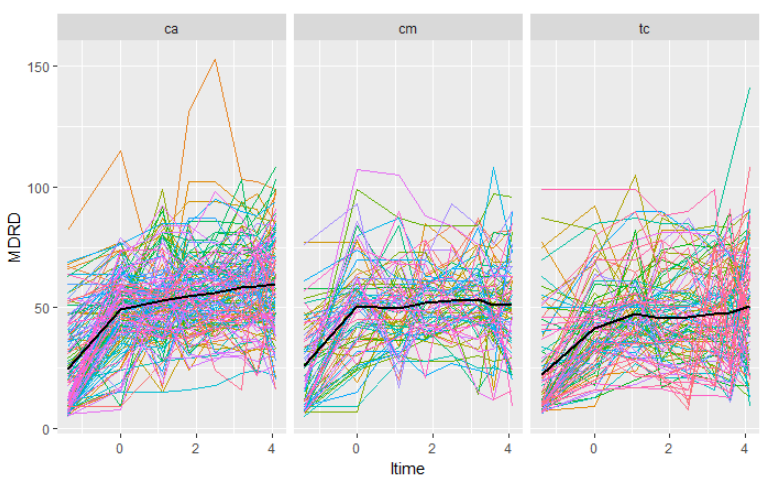
\includegraphics[height=0.4\textheight, width=\textwidth]{pictures/spaghetti.png}
\caption{Spaghetti plot of the data in different therapy groups with mean as black line} \label{spaghetti}
\end{figure}
We see slight differences in mean curves that confirm the results derived from values of coefficients. First, we can see that the level of MDRD is lower for each time point for therapy cm and tc in comparison to ca. Additionally the curve for therapy tc achieves its peak (the level from which it stops changing rapidly) later than the others and then the level of MDRD starts dropping slightly.

\subsection{Further time structure analysis}

After deriving the most adequate of considered mixed models we take a deeper look on the time structure. We change the growth model by including more and more complicated time equations. We perform calculations on cubic time and $time^4$, however the calculations for the last one do not converge. We use likelihood ratio test to choose the more adequate model between quadratic and cubic growth model. Because of p-value which is $< 0.0001$ we conclude that the cubic model fits our data best.

\subsection{Normality of random effects}

\begin{figure}[H] 
\centering
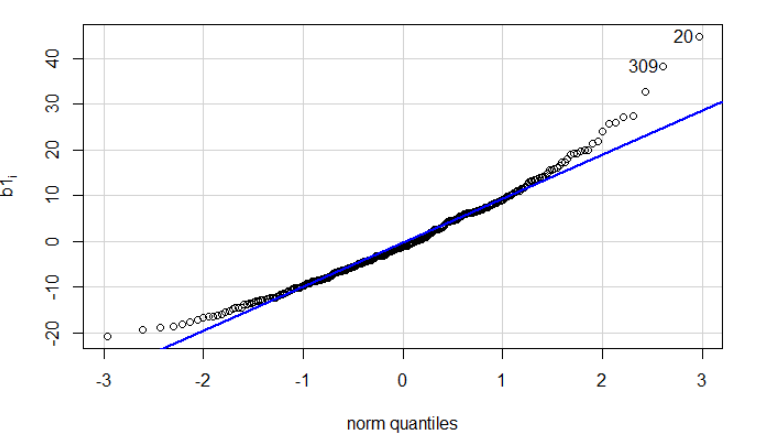
\includegraphics[height=0.25\textheight, width=0.45\textwidth]{pictures/b1.png}
\hfill
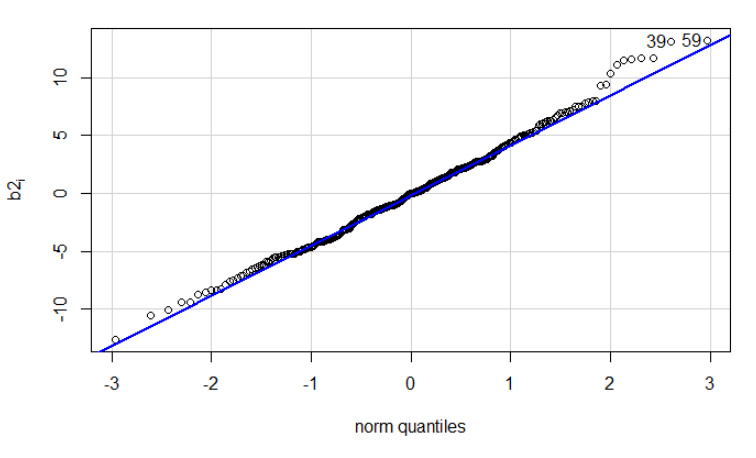
\includegraphics[height=0.25\textheight, width=0.45\textwidth]{pictures/b2.png}
\vfill
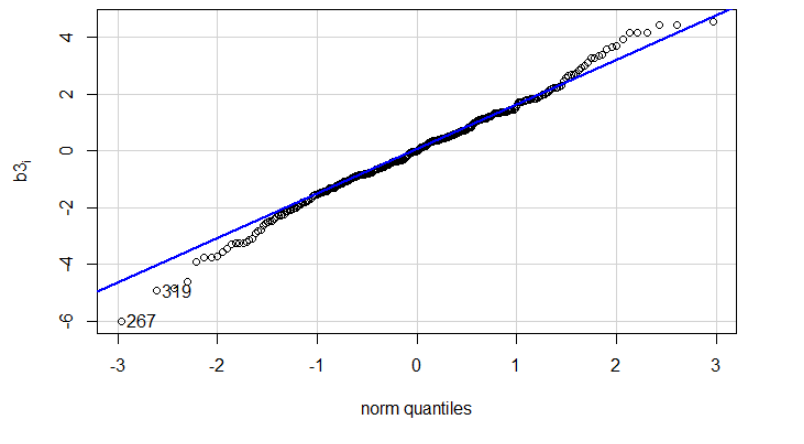
\includegraphics[height=0.25\textheight, width=0.45\textwidth]{pictures/b3.png}
\hfill
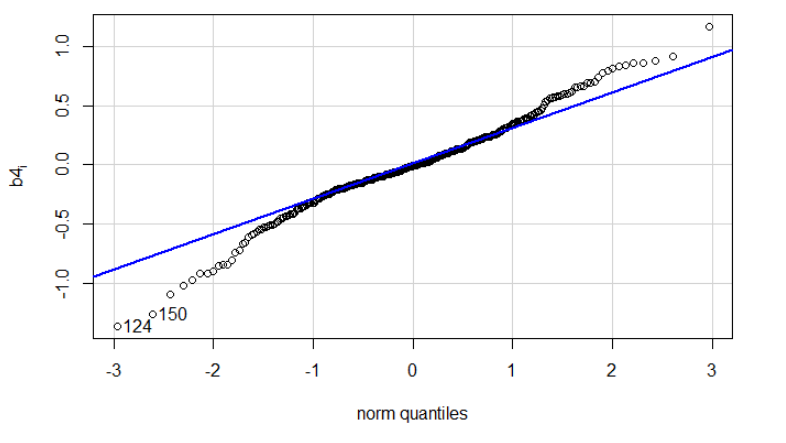
\includegraphics[height=0.25\textheight, width=0.45\textwidth]{pictures/b4.png}

\caption{Quantile diagrams for random effects from cubic growth model. First row: $b_{1i}, b_{2i}$, second row $b_{3i}$ and $b_{4i}$ (cubic time term)} \label{qq}
\end{figure}

Figure \ref{qq} presents four QQplots - the diagrams that show how far from normality the random effects are. It is useful for model diagnostics. We can observe that $b_{i2}$ which stands for linear slope fits the normal distributions very well. Other effects also fit the quantile line quite well, however they have more problems with a proper fit on tails. Especially for cubic term the deviations are noticeable. However, for now we stay with this model and leave it for further fit assessment in section \ref{asses}.

\section{Neural network for prediction}

As stated in the introduction we are also interested in prediction power of our models. Therefore we will compare our models with currently best available black-box predictor: neural network.

\subsection{Basics of neural networks}

The idea of artificial neural networks (ANN) is loosely based on the human brain. A real neural network consists of simple units called neurons. How do they work? Simplifying, we can say that a signal comes to a neuron through dendrites and then if it is "strong" enough it is passed to the following cells. One neuron can receive a signal from many neurons and pass it further to many others. The same scheme is used by ANN. An artificial neuron is a small computational unit connected with (possibly) many others. A more detailed description of the idea can be found in \cite{NN}. In the picture below we present an artificial neuron.

\begin{figure}[H]
\centering
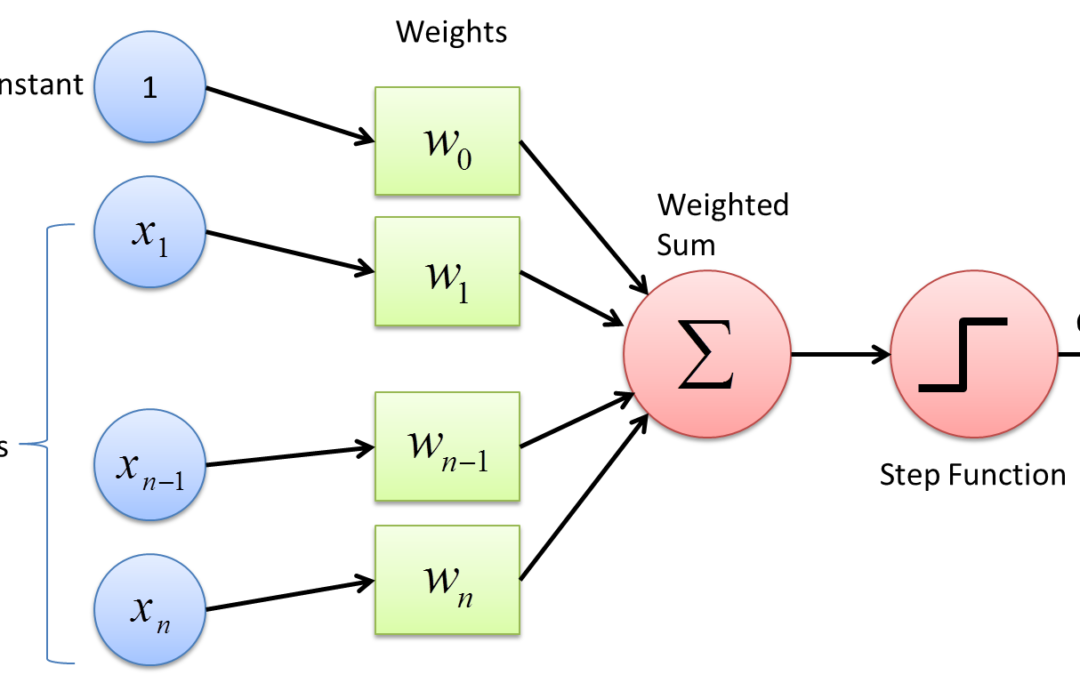
\includegraphics[width=\textwidth]{pictures/perceptron.png}
\caption{A single neuron of an artificial neural net}
\end{figure}

It consists of weights and an activation function. Mathematically speaking a one neuron calculates a function $f(x) = \sigma(W \cdot x)$, where $x = (1, x_1, \ldots, x_n)$ is the input vector (signal coming from dendrites), $W = (w_0, w_1, \ldots, w_n)$ are weights, $\cdot$ denotes dot product and $\sigma$ is an activation function which decide if the neuron "fires" - passes the signal further and/or squeezes the result. A two very popular examples of activation functions are sigmoid $\left(\sigma(x) = \frac{1}{1+e^{-x}}\right)$ and ReLU $\left(\sigma(x) = max(0,x)\right)$. One neuron has of course limited capabilities but an ANN consists of lots of neurons splitted to layers. The neurons within a single layer are not connected. The connections appear between neurons in  different layers. The  number of neurons in each layer and how they are connected are called the network architecture. Having these multiple connections between neurons allows the ANN to model very complicated nonlinear dependencies between input variables without any further assumptions, for example about the covariance structure. Even for two layers it would not be easy to write the formula for the output of ANN. 

The dimensionality of the output allows us to exploit neural networks in different problems. If we compute only one number, we get a solution for a regression problem. If we want to classify the data, we can have $k$ output neurons, where $k$ is the number of classes and each output would represent a probability of belonging to given class. Of course in order to ensure that these values fall into $[0,1]$ interval we have to use SOFTMAX layer before returning the results. Adding more neurons and layers gives us the possibility to model more and more complicated functions. However, this also causes exponential growth of the number of parameters (weights) in our model. Therefore finding their optimal (for example for mean squared error criterion) values is in fact intractable. Therefore, one more time we go back to brain analogy - humans can learn and this process is based on creating new connections between neurons, new neurons or strengthening existing links. In case of ANNs only the last feature is available: we want the weights of the network to be learnable. That is the reason why neural nets require a great amount of training data - it is used to adjust the weights which are usually initialized from a normal distribution with mean $0$. In order for neural network to learn we have to provide a training data set where each observation has a desired class(classification)/value(regression) and a penalty function $L$ (for example mean squared error or cross-entropy). Then during training we take advantage of a process called backpropagation. We feed the network with an observation $x$ and get result $f(x)$. We also calculate the penalty $L(f(x),x)$. Now we adjust the weights to lower the penalty: for each weight $w_i$ we change it slightly in the direction opposite to the gradient of $L$ by $w_i$. Formally:
$$
w_i = w_i - \alpha \frac{\partial L(f(x),x)}{\partial w_i}
$$
where $\alpha$ is a parameter called learning rate which is usually decreasing with the number of observation fed to the neural net. This algorithm of adjusting the weights is called gradient descent.

\subsection{Neural network for $kidney$ data set}

We try constructing a simple neural net which will be able to predict the value of $MDRD$ based on some features for each patient. Due to the limited number of patients the exploited network has to be small (few neurons/layers) and use only a subset of features for each patient. Otherwise the gradient descent algorithm would not be able to converge. By default ANN can include only numerical values as inputs. Therefore, for simplicity we do not feed our network with factors. We decide to use only $donor.age$, $bpl.drugs$ and $time$ as an input to our neural network. In the picture we below we present our network's architecture.

\begin{figure}[H]
\centering
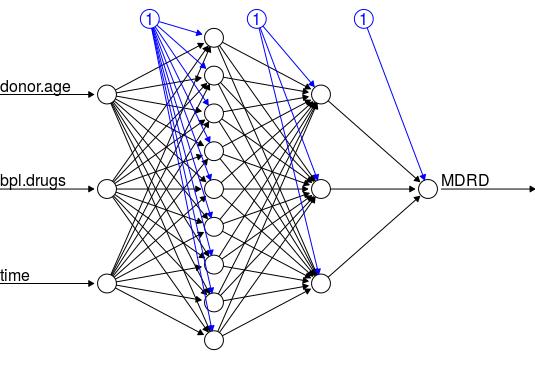
\includegraphics[width=\textwidth]{pictures/nn.png}
\caption{Used neural net architecture}
\end{figure}

It consists of two hidden layers of size $9,3$ respectively. Our architecture is fully connected (in neighboring layers all neurons are connected with each other). We use $threshold=0.1$ and standard $rprop+$ optimization method, mean squared error as a penalty function and sigmoid as activation for each neuron. For a description of the parameter check \cite{nn_pack}.

\section{Analysis and interpretation of results} \label{asses}

Due to the fact that the input for a neural network should be normalized, after obtaining predictions from our network we rescale them, so that they are comparable with the results from other models. We normalize our data by subtracting column mean and dividing by standard deviation for each column. 

We compare efficiency of six different models on our data set:
\begin{itemize}
\item Mixed effects model with quadratic time term (\textbf{Mixed(q.)})
\item Mixed effects model with cubic time term (\textbf{Mixed(c.)})
\item Chosen simpler fixed effects model with $time, donor.age$, $ therapy, time:therapy$ interaction and $bpl.drugs$ as explanatory variables. (\textbf{Fixed(s.)})
\item Fixed effects model with the same explanatory variables as the previous one but with quadratic time trend (\textbf{Fixed(q.)})
\item Full (most general) fixed effects model (\textbf{Fixed(f.)})
\item Neural network from section 4 (\textbf{NNet})
\end{itemize}
We use quadratic and cubic time terms mixed effects model because the experiments have shown that they are quite competitive. We also use full fixed effect model and the model chosen in our statistical analysis in section 2. Additionally, although as described in section 2 using fixed effects model with quadratic time trend is not defensible for our data, we want to check how such significant reduction in number of parameters in the model influences prediction power.

We use 4 different measures of model assessment: Akaike Information Criterion, percentage of variance in the data set explained by the model measured using the formula:
$$
perc.var(model) = \left(1 - \frac{Var(residuals(model))}{Var(MDRD)}\right) \cdot 100
$$
where $Var$ denotes variance. We also use the mean squared error of prediction on the training set and test set. The values of these criteria are calculated using the following procedure:
\begin{itemize}
\item We split our data set to training set ($80\%$ of the data) and test set ($20\%$ of the data) randomly (we sample without replacement indices of patients which are put to the test set)
\item We fit all models from the table on the training set and report their AIC, percentage of explained variance and prediction error on this set
\item For neural network we perform additional step of normalizing data before training (and then rescaling the results) 
\item We then predict and report prediction errors on the test set for each model
\item To make tour analysis comprehensive we apply the described scheme five times and in the table we report the mean of these five repetitions
\end{itemize}

We present the results in the table below.

\begin{table}[H]
\caption{Comparison of different models}
\begin{threeparttable}
\centering
\begin{adjustbox}{max width=\textwidth}
\begin{tabular}{rrrrrrr}
 \headrow
 & Mixed(q.) & Mixed(c.) & Fixed(s.) & Fixed(q.) & Fixed(f.) & NNet \\ 

AIC & 17535.86 & 17445.14 & 17173.05 & 17298.67 & 17151.87 &  \\ 
  \% var. & 76.66 & 81.78 & 32.84 & 31.13 & 33.92 &  20.80\\ 
  Train err. & 97.61 & 76.19 & 280.92 & 288.27 & 276.39 & 331.06 \\ 
  Test err. & 616.84 & 639.27 & 504.10 & 490.12 & 510.71 & 452.92 \\ 
   \hline
\end{tabular}
\end{adjustbox}
\end{threeparttable}
\end{table}

\paragraph{AIC}

First we take a look at a model selection criterion AIC. We notice that mixed effects models have significantly higher value of the criterion than fixed effects models. When it comes to fixed effects model although statistical tests shown that full model is not significantly better than the simple one the value of AIC indicates that it is the best model for our data. 

\paragraph{Percentage of explained variance}

We also compare percentage of variance explained by each of the models. Looking at the fixed model we can again see the same effect as for AIC: full model is the best, simple a little worse and quadratic the worst of these three. However the differences are slight and they all explain around $32$\% of variance in the data set which is quite good result for medical data. For neural network the percentage of explained variance is the smallest - only $21\%$.

On the other hand, we can notice that the percentage of explained variance is much larger for mixed effects models. It is caused by their formulation. The residuals are not measured from population curve (as in the case of fixed effects model) but from the curve fitted individually for each patient by introducing random effects. Therefore such difference between mixed and fixed effects is not surprising. Nonetheless, we claim that this is a valid criterion for model comparison. To support this statement we focus on the interpretation on random effects. Especially in medical data (as we write in the previous paragraph) we are content with $32$\% of variance explained. This is due to the fact that there are many more latent variables that significantly influence our response (for example genomes, diet, environment, lifestyle etc.) about which information are either very hard or even impossible to collect. The random effects allow us to incorporate our knowledge about existence of these latent variables in the model. Hence, in terms of explained variance the best model is Mixed(c.) which also beats the Mixed(q.) model by $5$\%. 
\paragraph{Prediction}
Another criterion considered is the efficiency on the training and test set. This is very important measure, because models with reasonably high prediction capabilities can be used to model MDRD for future patient. Basing on such prediction with different parameters the proper therapy or number of blood pressure lowering drugs can be chosen. On the training set mixed effects models have no competition. This is caused by the effects described in previous paragraph. In fact training error and percentage of variance explained are directly connected - $MSE_{train} = Var(residuals(model))$. However, what is of main interest is the prediction error on the test set, because it is the estimate of how good our model will be on the new data. The mixed effects models are significantly worse than all the other. The reason is that when predicting the values of response for new data no random effect is fitted and it only provides the value calculated from the population curve. For fixed effects models the results are little better. We can see that the Fixed(q.) model has the lowest prediction error due to having much fewer parameters than the other two. Therefore the overfiting effect (difference between train error and test error) is smaller but still significant. We can see that at least in case of our fixed and mixed effects models, the fewer parameters in the model, the lower prediction errors obtained. 

Although the neural network is the worst model when comparing the training errors and explained variance, it has significantly lowest prediction error and overfitting effect among all considered models. It is worth noticing that the architecture was chosen almost arbitrarily, we used only fully connected layers, default network parameters and no hyperparameters (for example learning rate) tuning and in spite of this fact neural network provides better prediction than the sophisticated linear models for longitudinal data. Therefore based on the prediction criterion our neural network is the best model. However, we have to note that mean squared error of $450$ is equivalent to mean deviation of $21$ which is very high for MDRD variable which has the mean around $46$. As a result, none of the models is usable in terms of prediction. 

\paragraph{Summary}

In our analysis we compared and investigated the properties on different models on the $kidney$ data set. We used fixed effects, mixed effects model and a neural network. We used different criteria to measure their effectiveness and fitness. Unfortunately, in terms of prediction we didn't obtain reasonable model. Nonetheless, mixed and fixed effects models allowed us to find some dependencies between our variables. Therefore, we would claim that our mixed effects models fit best to our data among considered models, because they allow us to incorporate the effect of latent variables which are very common in medical studies.

\newpage
\bibliography{sample}


\end{document}
